\documentclass[10pt]{article}
\usepackage{NotesTeX}
\usepackage{lipsum}
\usepackage{tensor}
\usepackage{amsmath,amsthm,amssymb}
\usepackage{hyperref}
\usepackage{indentfirst}
\usepackage{mathrsfs}
\usepackage{graphicx}

\newcommand{\bs}{\textbackslash}


\title{{\Huge General Relativity}\\{\Large{Class 37 --- April 24, 2020}}} %replace with class number
\author{Kunhao Zhong}

\emailAdd{maxzhong@utexas.edu} %replace with your email
\begin{document}
    \maketitle
    \flushbottom
    \newpage
    \pagestyle{fancynotes}
    \part{Gravitational Waves}

\section{Wave Solution to the Einstein's Equation}

Gravitational wave is one of the most important prediction of general relativity. It is the solution to the source-free, linearized Einstein's equation, in Lorentz gauge:

\begin{equation}\label{eq: wave_eqn}
\begin{aligned}
\partial^{\alpha} \bar{h}_{\alpha \mu}&=0\\
\partial^{\alpha} \partial_{\alpha} \bar{h}_{\mu\nu}&=0
\end{aligned}
\end{equation}

We can take the general solution to the wave equation $ \square \bar{h}_{\mu\nu}=0 $ as:
\begin{equation}\label{eq: wave_form}
\bar{h}_{\mu\nu}=C_{\mu\nu} \mathrm{e}^{\mathrm{i} k_{\sigma}x^{\sigma}}
\end{equation}
where
\begin{equation}\label{eq: kx_component}
k_{\sigma}x^{\sigma}=k_0 t+k_1 x+ k_2 y+k_3 z
\end{equation}

The requirement on this form of solution is given by the wave equation:

\begin{equation}\label{eq: null_condition}
\begin{aligned}
0=\square \bar{h}_{\mu\nu}&=C_{\mu\nu} \partial^{\alpha} \partial _{\alpha} \mathrm{e}^{\mathrm{i}k_\sigma x^\sigma}\\
&=C_{\mu\nu}\partial^\alpha (\mathrm{e}^{\mathrm{i} k_\sigma x^\sigma} \mathrm{i}k_\sigma \partial_\alpha x^\sigma)\\
&=C_{\mu\nu}\mathrm{i}k_\alpha \partial^\alpha (\mathrm{e}^{\mathrm{i}k_\sigma x^\sigma})\\
&=-C_{\mu\nu} k_\alpha k^\alpha \mathrm{e}^{\mathrm{i} k_\sigma x^\sigma}
\end{aligned}
\end{equation}
and this requires $ k_\alpha k^\alpha=0 $, or $ k^\mu $ to be a null vector. This tells us that the gravitational waves travels at the speed of light.

Similarly, the Lorentz gauge condition requires:
\begin{equation}\label{transverse_condition}
\partial^\alpha \bar{h}_{\alpha\mu}=\mathrm{i} k^\alpha C_{\alpha\mu} \mathrm{e}^{\mathrm{i} k_\sigma x^\sigma}=0
\end{equation}
and this gives $ k^\alpha C_{\alpha \nu}=0 $. This is called the transverse condition, in analogy to the condition in electromagnetic waves that $ E $ and $ B $ are always orthogonal along the propagation.

We can further simplify our solution by assuming the wave is propagating thought the $ z $ direction:
\begin{equation}\label{eq: z_direction}
\begin{aligned}
k_\mu&=(\omega,0,0,\omega)\\
k_\sigma x^\sigma&=-\omega t+\omega z=-\omega(t-z)
\end{aligned}
\end{equation}
which tells us that the wave is only a function of the retarded time $ t_r=t-z $. And we will adopt this assumption through the chapter.

Since $ h_{\mu\nu} $ is only a function or retarded time, any derivative other than $ t $ or $ z $ vanishes. This reduce the Lorentz gauge condition to:
\begin{equation}\label{eq: Lorentz_gauge_condition_1}
-\partial_t \bar{h}_{t \nu}+\partial_z \bar{h}_{z \nu}=0
\end{equation}
which leads to:
\begin{equation}\label{eq: Lorentz_gauge_condition_2}
-\dot{\bar{h}}_{0 \nu}-\dot{\bar{h}}_{z \nu}=0
\end{equation}
where the dot means derivative with respect to the argument $ t_r $. Take the integral and gives:
\begin{equation}\label{eq: Lorentz_gauge_condition_3}
\bar{h}_{0 \nu}=-\bar{h}_{z \nu}
\end{equation}
which is a very useful equation because this means wherever we solve the spacial components, we automatically get the time component. 

We will explore more on the homework assignment for the transverse traceless gauge (TT), or radiation gauge, in which $ \bar{h}_{\mu\nu}=h_{\mu\nu} $ since its traceless. And we can also set $ h_{tt}=h_{zz}=0 $ in this gauge, which left the perturbation metric as:
\begin{equation}\label{eq: metric_TT}
h_{\mu\nu}=
\begin{pmatrix}
0 & 0 & 0 & 0 \\ 
0 & h_{xx} & h_{xy} & 0 \\ 
0 & h_{xy} & -h_{xx} & 0 \\ 
0 & 0 & 0 & 0
\end{pmatrix}
\end{equation}

We can see from the above equation that there are two independent component of $ h_{\mu\nu} $, corresponding to two polarization. And we can name them as:
\begin{equation}\label{eq: polarization}
\begin{aligned}
h_{+} &\equiv h_{xx}\\
h_{\times} &\equiv h_{xy}
\end{aligned}
\end{equation}

We can do the similar transformation in frequency domain, which will set:
\begin{equation}\label{key}
C_{\mu\nu}=
\begin{pmatrix}
0 & 0 & 0 & 0 \\ 
0 & C_{11} & C_{12} & 0 \\ 
0 & C_{12} & -C_{11} & 0 \\ 
0 & 0 & 0 & 0
\end{pmatrix}
\end{equation}

The two kinds of polarization are two independent solution to the Einstein's equation, and a general solution is any combination of them since Einstein's equation is linearized. This is exactly the same thing as electromagnetic wave theory  because we are solving the same type of equation.

\section{Effect of Gravitational Waves}
We now have the solution to the Einstein's equation. Since we know the metric tells us everything about the geometry of the space-time, it is natural to ask: What do the gravitational waves do when they propagate though particles?

We consider particles at rest, as shown in figure 1. 
\begin{figure}
	\centering
	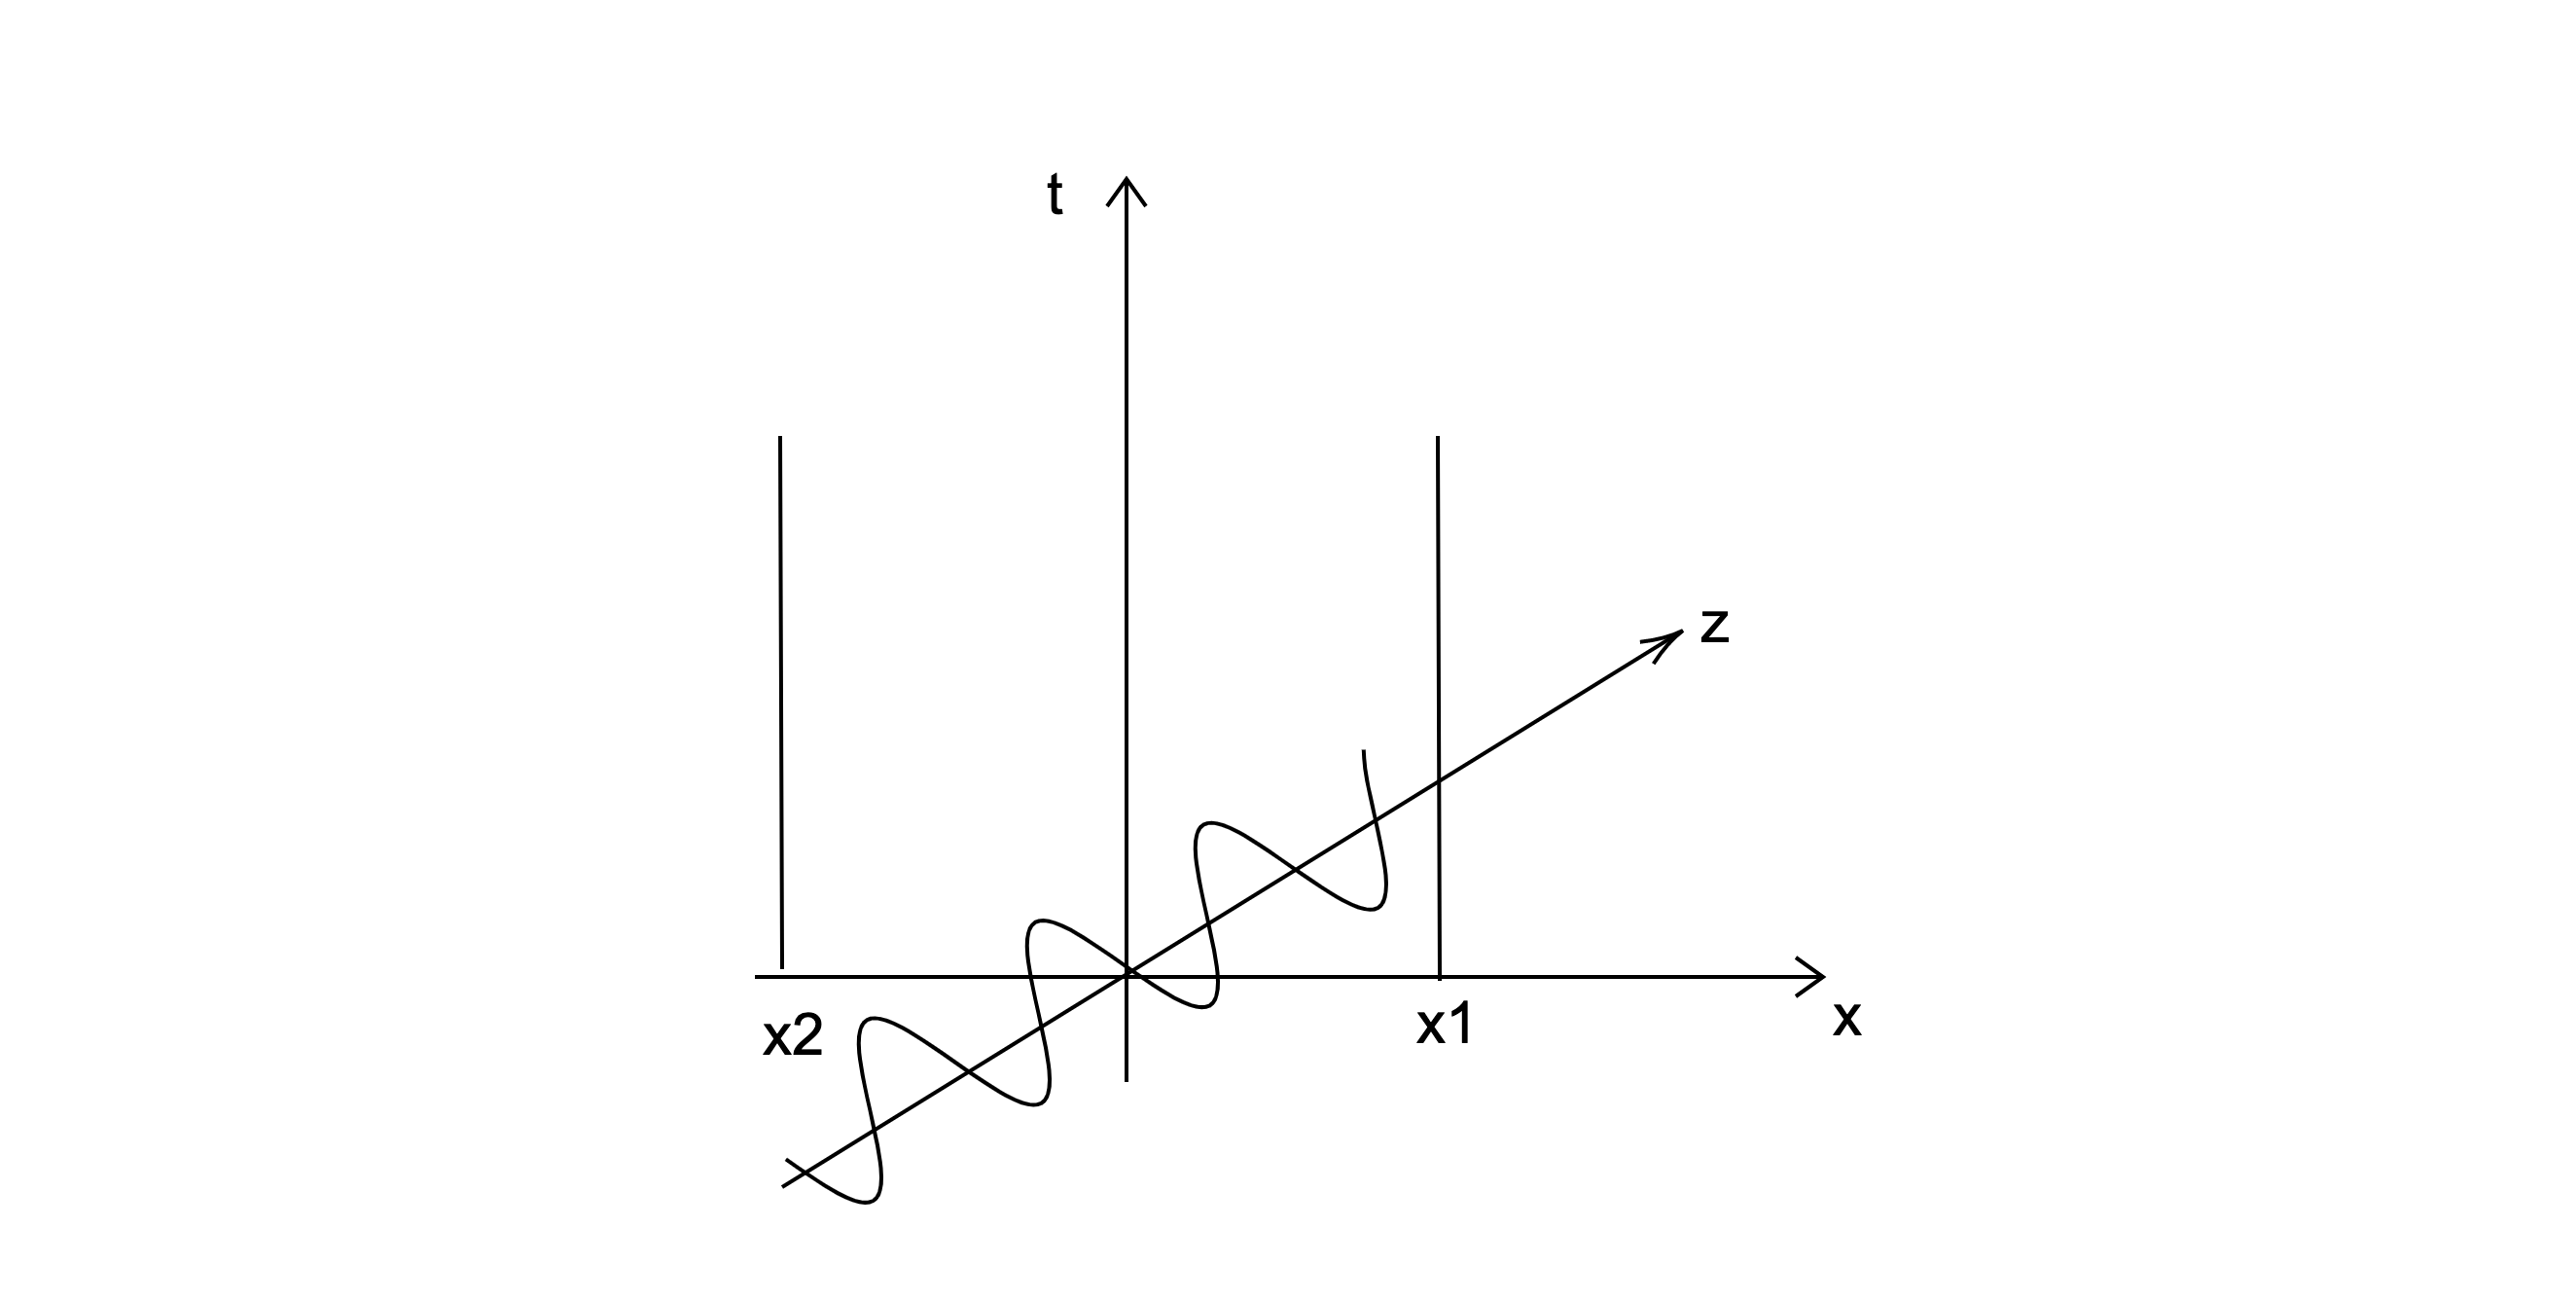
\includegraphics[width=0.9\linewidth]{particle@rest.png}
	\caption{Consider particles at rest, and gravitational waves travel trough them}
	\label{fig: particle at rest}
\end{figure}
The back ground geometry are know governed by:
\begin{equation}\label{eq: background metric}
g_{mu\nu}=\eta_{\mu\nu}+h_{\mu\nu}
\end{equation}
where$ h_{\mu\nu} $ is the solution to the wave equation. Assume the particle is initially at rest, so
\begin{equation}\label{eq: initial_velocity}
U^\mu |_{\tau=0}=(1,0,0,0)
\end{equation}
and the motion equation is then
\begin{equation}\label{eq: motion equation}
\dfrac{\mathrm{d^2 x^{\mathrm{i}}}}{\mathrm{d} \tau^2}|_{\tau=0}=-\Gamma^{\rm i}_{\hphantom{\rm i}\alpha\beta}  U^\alpha U^\beta |_{\tau=0}=-\eta^{\rm i \nu} (\partial_0 h^{TT}_{0 \nu}+\partial h^{TT}_{0 \nu}- \partial h^{TT}_{00})=0
\end{equation}
The last equality holds because the derivative of those components equals zero(the superscript "TT" means a tensor in transverse traceless gauge). This tells us that the acceleration of a particle is zero, and since it has zero initial velocity, the particle will stay at rest. Does this mean the gravitational wave will have no effect on the particles? It turns out our calculation is in a special coordinate system that coordinates change with the particle, and the particle just appears not to move.

To see the effect of gravitational waves, we consider the proper distance between two particles, as shown in figure 2.
\begin{figure}
	\centering
	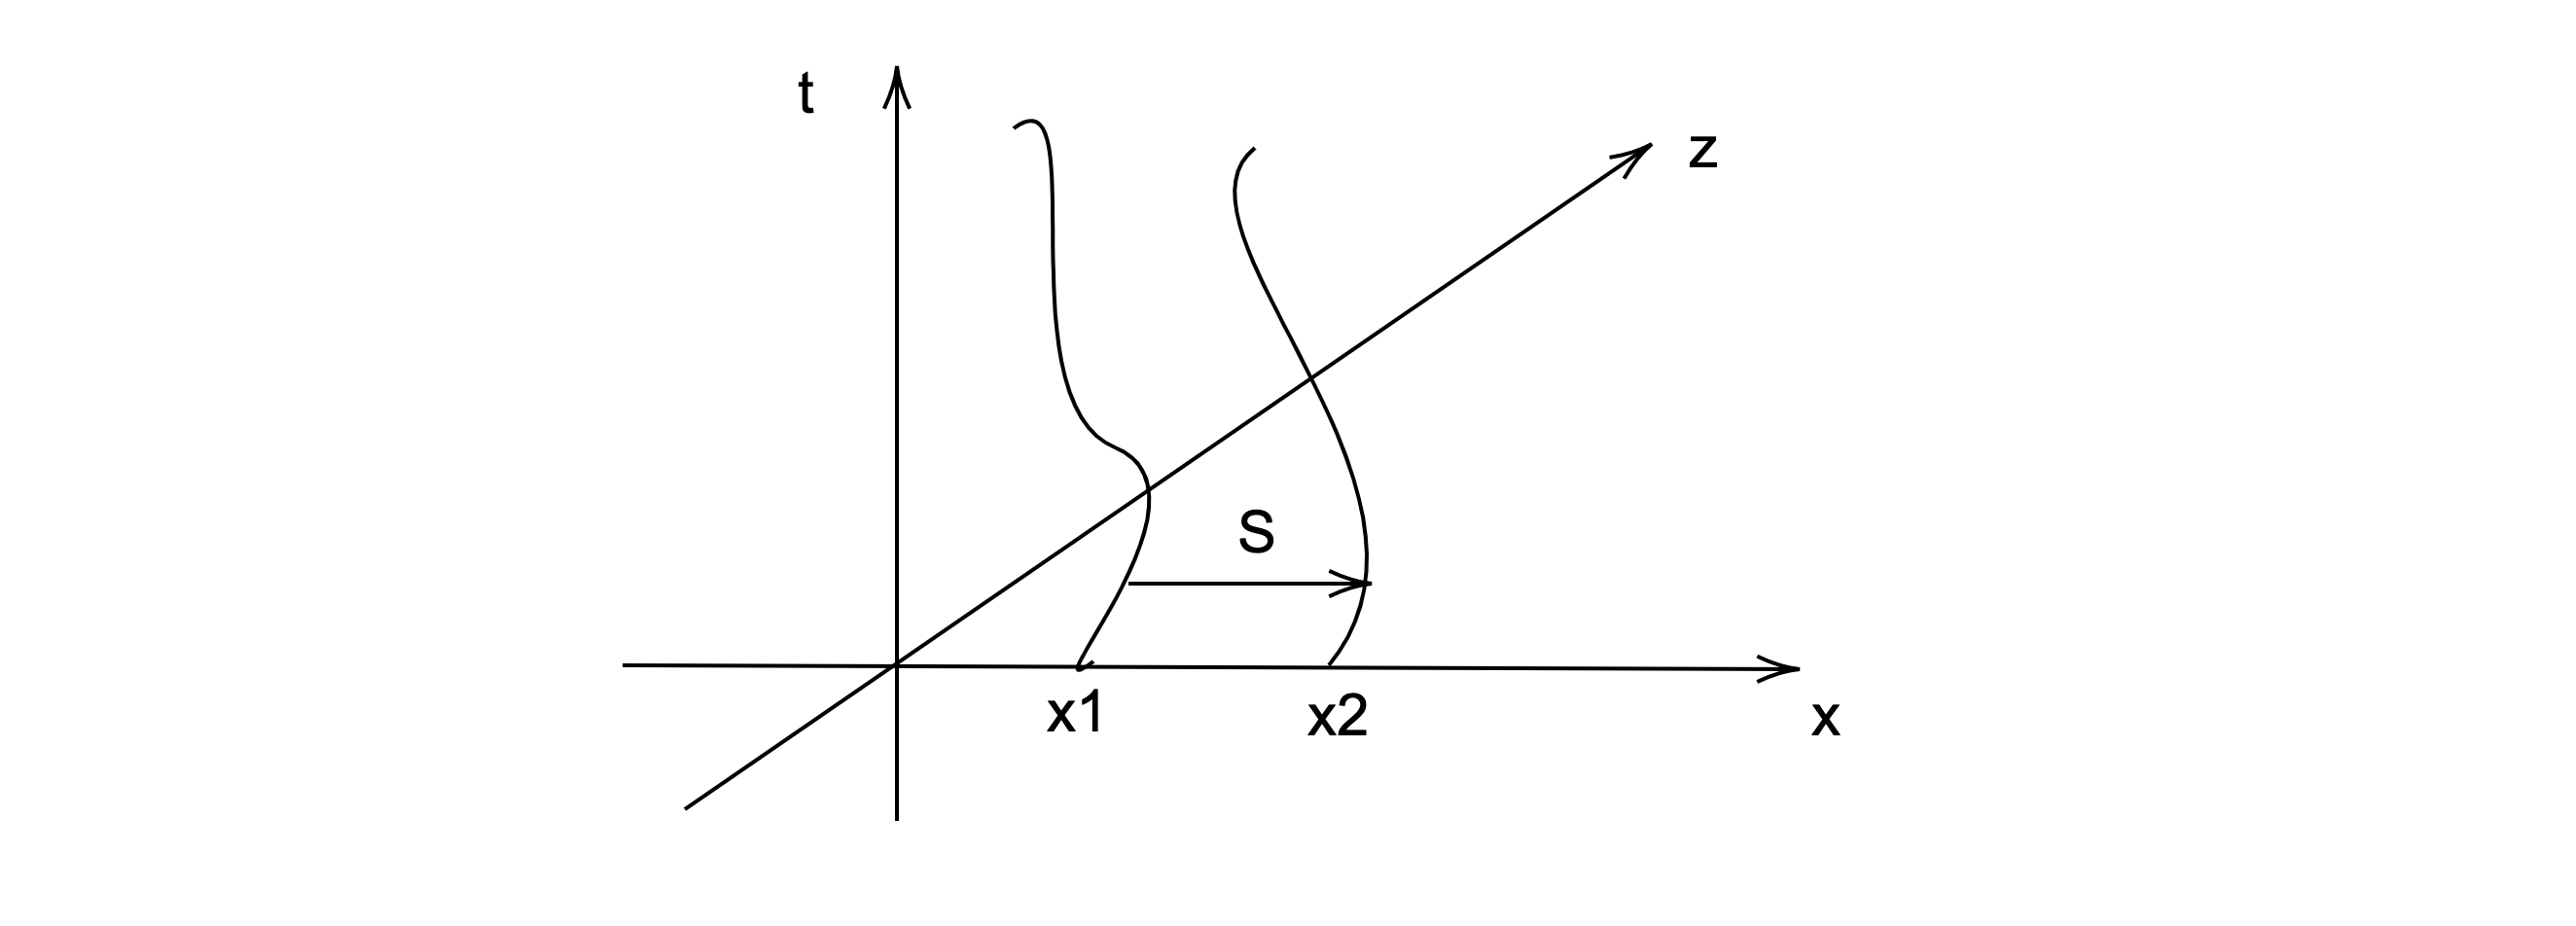
\includegraphics[width=1\linewidth]{proper_distance}
	\caption{Proper distance between two particles when a gravitational wave propagate through them}
	\label{fig:properdistance}
\end{figure}
\begin{equation}\label{eq: proper_distance}
S=\int_{x_1}^{x_2} \sqrt{g_{xx} \mathrm{d} x^2}=\int_{x_1}^{x_2}\sqrt{1+h^{TT}_{+}} \mathrm{d} x \approx (x_2-x_1)(1+\dfrac{1}{2} h^{TT}_+(t))
\end{equation}
here we consider $ h_+ $ polarization (in fact, if we assume the particles are on the x axis, the $ h_\times $ will have no effect because they have the same y coordinates $ d y=0 $). We can see from this equation that the proper distance between two particles are largely unchanged, with a oscillating term $ \dfrac{1}{2} h^{TT}_+(t) $.

The geodesic deviation equation can tell us more information
\begin{equation}\label{eq: geodesic_deviation_eqn}
\dfrac{\mathrm{D}^2 S^\mu}{\mathrm{d}\tau^2}
=U^\alpha \Delta_\alpha (U^\beta \Delta_\beta S^u)= R^{\mu}_{\hphantom{\mu}\nu\rho\sigma} U^\nu U^\rho S^\sigma
\end{equation}
since the Riemann tensor is of order $ h_{\mu\nu} $, we can approximate on the right hand side with $ t $ in replace of $ \tau $. We can calculate $ R_{\nu 0 0 \nu}=\dfrac{1}{2} \ddot{h}^{TT}_{\mu\nu} $, and we omit the detail of calculation here since every necessary information is contained in the metric. By substitute this component into the geodesic deviation equation
\begin{equation}\label{eq: compenent_geodesic_deviation}
\partial^2_t S^\mu= \dfrac{1}{2} S^\sigma \partial^2_t h^\mu_{\hphantom{\mu}\sigma}
\end{equation}
We can solve this equation analytically. Consider only $ h_+ $ polarization.
\begin{equation}\label{key}
\ddot{h}^\mu_\sigma S^\sigma
=
\begin{pmatrix}
0 & 0 & 0 & 0 \\ 
0 & \ddot{h_+} & 0 & 0 \\ 
0 & 0 & -\ddot{h_+} & 0 \\ 
0 & 0 & 0 & 0
\end{pmatrix}
\begin{pmatrix}
S^0 \\ 
S^1 \\ 
S^2\\ 
S^3
\end{pmatrix}
=
\begin{pmatrix}
0 \\ 
 \ddot{h}_+S^1 \\ 
- \ddot{h}_+S^2\\ 
0
\end{pmatrix}
\end{equation}
Then it gives the following equations:
\begin{equation}\label{eq: geo_deiviation_component}
\ddot{S^1}=\dfrac{1}{2} S^1 \ddot{h}_+
\end{equation}
with the approximation$ \ddot{(S^1 h_+)}=\ddot{S^1} h_+ +S^1 \ddot{h}_+ \approx S^1 \ddot{h}_+ $, we can integrate this equation directly with some boundary conditions
\begin{equation}\label{eq: sln to S1}
S^1=(1+\dfrac{1}{2} h_+(t-z)) S^1(t=0)
\end{equation}
Similar calculation generates solution to $ S^1 $ as well as $ S^\mu $ in $ h_\times $ polarization. In summary
\begin{equation}\label{eq: geo_deviation_hplus}
\begin{aligned}
S^1&=(1+\dfrac{1}{2} h_+(t-z)) S^1(t=0)\\
S^2&=(1-\dfrac{1}{2} h_+(t-z)) S^2(t=0)
\end{aligned}
\end{equation}
for $ h_+ $ polarization and
\begin{equation}\label{eq: geo_deviation_hcross}
\begin{aligned}
S^1&=S^1(0)+\dfrac{1}{2} S^2(0) h_\times (t-z)\\
S^2&=S^2(0)+\dfrac{1}{2} S^1(0) h_\times (t-z)
\end{aligned}
\end{equation}
The oscillation modes are shown in figure 3
\begin{figure}
	\centering
	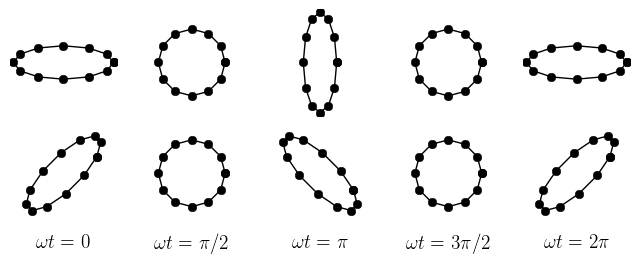
\includegraphics[width=0.7\linewidth]{gw_ring.png}
	\caption{Tidal effect of two modes of gravitational waves}
	\label{fig:gwring}
\end{figure}

The geodesic deviation equation
\begin{equation}\label{eq: geo_dev_ij}
R_{i,0,j,0}=\dfrac{1}{2} \ddot{h}^{TT}_{ij} \equiv \mathcal{E}_{ij}
\end{equation}
is exceptionally important because the Riemann tensor is gauge invariant and we can integrate directly to get
\begin{equation}\label{eq: reverse_calculation}
h^{TT}_{ij}=-2 \int\mathrm{d}t \int\mathrm{d}t \mathcal{E}_{ij}
\end{equation} 


\section{Resonant Bar Detector}
The method of resonant bar detector was first proposed by Joseph Weber, who claimed the detection of gravitational waves in the 1970s. Although it was widely considered that he's results has no evidence of the detection of gravitational waves, he was one of the pioneers in gravitational wave detection. A detailed review can by found at \textit{Douglass and Braginsky 1979} \footnote{Douglass, D.H., Braginsky, V.B. Israel, W. (Ed.). (1979). Gravitational-radiation experiments. United Kingdom: University Press.}. We will introduce the ideas of resonant bar detector in this section.

The main ideas is pretty simple. Since the gravitational waves will oscillate the proper distance between particles, we should expect an external force on two particles attached on two sides of a spring. Consider two particles of equal mass $ m $ attached on a spring
\begin{equation}\label{eq: motion_of_spring}
\begin{aligned}
m \ddot{x}_1&=k (l-l_0)\\
m \ddot{x}_2&=-k (l-l_0)
\end{aligned}
\end{equation}
the proper distance with the effect of gravitational wave perturbation becomes:
\begin{equation}\label{eq: proper_distance_spring}
\begin{aligned}
l(t)&=\int_{x_1(t)}^{x_2(t)} \sqrt{(1-h_+(t))} \mathrm{d}\\
&=(x_2-x_1) +\dfrac{1}{2} h_+(x_2-x_1)+\mathcal{O}(h^2)
\end{aligned}
\end{equation}

Let $ q \equiv l-l_0 $. Substituting the solution of $ l(t) $ and the spring motion $ x(t) $ gives
 \begin{equation}\label{eq: derive_motion_q}
 \begin{aligned}
 q &\equiv l-l_0 = x_2-x_1 +\dfrac{1}{2} h_+ l_0 - l_0\\
 \ddot{q} &= \ddot{x_2}-\ddot{x_1}+\dfrac{1}{2} \ddot{h}_+  l_0\\
 &=(-\dfrac{\omega_0^2}{2}-\dfrac{\omega_0^2}{2})(l-l_))+\dfrac{1}{2} l_0 \ddot{h}_+
 \end{aligned}
 \end{equation}
or 
\begin{equation}\label{eq: motion_q}
\ddot{q}+\omega_0^2 q=\dfrac{1}{2} l_0 \ddot{h}_+
\end{equation}
which is of the standard form of a spring with external sinusoidal force with damping term
\begin{equation}\label{eq: standard_motion}
\ddot{q}+2 \gamma \dot{q}+ \omega_0^2 q=\dfrac{1}{2} l_0 \ddot{h}_+
\end{equation}
which has a standard solution
\begin{equation}\label{eq: sln_q}
q=R \cos (\Omega t+\phi)
\end{equation}
where
\begin{equation}\label{eq: R_term}
R=\dfrac{1}{2} \dfrac{\Omega^2 A l_0}{((\omega_0^2-\Omega^2)^2+4\Omega^2 \gamma^2)^{1/2}}
\end{equation}
If we can make $ \omega_0 \approx \Omega $, the resonance phenomenon will largely increase the oscillation of the bar and in theory we can use this to detect gravitational waves.

However, it turns out that this method is too difficult to achieve in reality. But it do lead the way to the invention of interferometer, and finally in 2017, LIGO managed to confirm the first case of gravitational wave generated from binary blackholes collision.
\begin{figure}
	\centering
	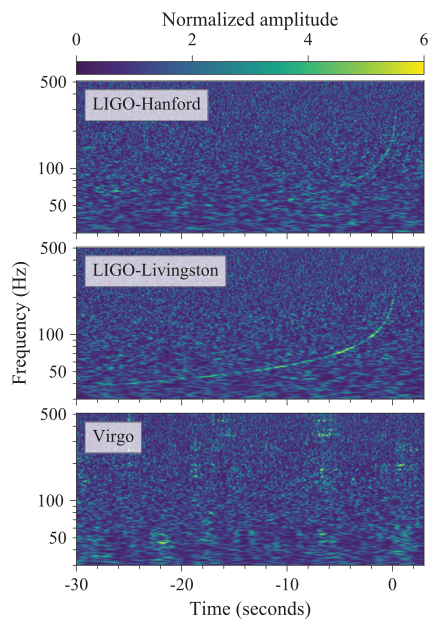
\includegraphics[width=0.7\linewidth]{GW170817}
	\caption{The first case of gravitational detection GW170817}
	\label{fig:gw170817}
\end{figure}




\end{document}